%%% Hlavní soubor. Zde se definují základní parametry a odkazuje se na ostatní části. %%%




%% Verze pro jednostranný tisk:
% Okraje: levý 40mm, pravý 25mm, horní a dolní 25mm
% (ale pozor, LaTeX si sám přidává 1in)
\documentclass[12pt,a4paper]{report}
\setlength\textwidth{145mm}
\setlength\textheight{247mm}
\setlength\oddsidemargin{15mm}
\setlength\evensidemargin{15mm}
\setlength\topmargin{0mm}
\setlength\headsep{0mm}
\setlength\headheight{0mm}
% \openright zařídí, aby následující text začínal na pravé straně knihy
\let\openright=\clearpage

\usepackage{setspace}
\onehalfspacing
%% Pokud tiskneme oboustranně:
% \documentclass[12pt,a4paper,twoside,openright]{report}
% \setlength\textwidth{145mm}
% \setlength\textheight{247mm}
% \setlength\oddsidemargin{15mm}
% \setlength\evensidemargin{0mm}
% \setlength\topmargin{0mm}
% \setlength\headsep{0mm}
% \setlength\headheight{0mm}
% \let\openright=\cleardoublepage

%% Použité kódování znaků: obvykle latin2, cp1250 nebo utf8:
\usepackage[utf8]{inputenc}

%% Ostatní balíčky
\usepackage{graphicx}
\usepackage{amsthm}
\usepackage{latexsym}
\usepackage{mathtools}
\newtheorem{mydef}{Definition}
%% Balíček hyperref, kterým jdou vyrábět klikací odkazy v PDF,
%% ale hlavně ho používáme k uložení metadat do PDF (včetně obsahu).
%% POZOR, nezapomeňte vyplnit jméno práce a autora.
\usepackage[unicode]{hyperref}   % Musí být za všemi ostatními balíčky



\hypersetup{pdftitle=Název práce}
\hypersetup{pdfauthor=Marcel Kikta}

%%% Drobné úpravy stylu

% Tato makra přesvědčují mírně ošklivým trikem LaTeX, aby hlavičky kapitol
% sázel příčetněji a nevynechával nad nimi spoustu místa. Směle ignorujte.
\makeatletter
\def\@makechapterhead#1{
  {\parindent \z@ \raggedright \normalfont
   \Huge\bfseries \thechapter. #1
   \par\nobreak
   \vskip 20\p@
}}
\def\@makeschapterhead#1{
  {\parindent \z@ \raggedright \normalfont
   \Huge\bfseries #1
   \par\nobreak
   \vskip 20\p@
}}
\makeatother



% Toto makro definuje kapitolu, která není očíslovaná, ale je uvedena v obsahu.
\def\chapwithtoc#1{
\chapter*{#1}
\addcontentsline{toc}{chapter}{#1}
}

\begin{document}

% Trochu volnější nastavení dělení slov, než je default.
\lefthyphenmin=2
\righthyphenmin=2

%%% Titulní strana práce

\pagestyle{empty}
\begin{center}

\large

Charles University in Prague

\medskip

Faculty of Mathematics and Physics

\vfill

{\bf\Large MASTER THESIS}

\vfill

\centerline{\mbox{
\includegraphics[width=60mm]{img/logo.pdf}}}

\vfill
\vspace{5mm}

{\LARGE Marcel Kikta}

\vspace{15mm}

% Název práce přesně podle zadání
{\LARGE\bfseries Evaluating relational queries in pipeline-based environment}

\vfill

% Název katedry nebo ústavu, kde byla práce oficiálně zadána
% (dle Organizační struktury MFF UK)
Department of Software Engineering

\vfill

\begin{tabular}{rl}

Supervisor of the master thesis: & David Bednárek \\
\noalign{\vspace{2mm}}
Study programme: & Software systems \\
\noalign{\vspace{2mm}}
Specialization: & Software engineering \\
\end{tabular}

\vfill

% Zde doplňte rok
Prague 2014

\end{center}

\newpage

%%% Následuje vevázaný list -- kopie podepsaného "Zadání diplomové práce".
%%% Toto zadání NENÍ součástí elektronické verze práce, nescanovat.

%%% Na tomto místě mohou být napsána případná poděkování (vedoucímu práce,
%%% konzultantovi, tomu, kdo zapůjčil software, literaturu apod.)

\openright

\noindent
Dedication.

\newpage

%%% Strana s čestným prohlášením k diplomové práci

\vglue 0pt plus 1fill

\noindent
I declare that I carried out this master thesis independently, and only with the cited
sources, literature and other professional sources.

\medskip\noindent
I understand that my work relates to the rights and obligations under the Act No.
121/2000 Coll., the Copyright Act, as amended, in particular the fact that the Charles
University in Prague has the right to conclude a license agreement on the use of this
work as a school work pursuant to Section 60 paragraph 1 of the Copyright Act.

\vspace{10mm}

\hbox{\hbox to 0.5\hsize{%
In ........ date ............
\hss}\hbox to 0.5\hsize{%
signature of the author
\hss}}

\vspace{20mm}
\newpage

%%% Povinná informační strana diplomové práce

\vbox to 0.5\vsize{
\setlength\parindent{0mm}
\setlength\parskip{5mm}

Název práce:
Vyhodnocování relačních dotazů v proudově orientovaném prostředí
% přesně dle zadání

Autor:
Marcel Kikta

Katedra:  % Případně Ústav:
Katedra softwarového inženýrství
% dle Organizační struktury MFF UK

Vedoucí diplomové práce:
RNDr. David Bednárek, Ph.D.
% dle Organizační struktury MFF UK, případně plný název pracoviště mimo MFF UK

Abstrakt:
% abstrakt v rozsahu 80-200 slov; nejedná se však o opis zadání diplomové práce

Klíčová slova:
SQL, Prěkladač, Relační algebra, Optimalizator, Bobox

\vss}\nobreak\vbox to 0.49\vsize{
\setlength\parindent{0mm}
\setlength\parskip{5mm}

Title:
% přesný překlad názvu práce v angličtině

Author:
Marcel Kikta

Department:
Název katedry či ústavu, kde byla práce oficiálně zadána
% dle Organizační struktury MFF UK v angličtině

Supervisor:
RNDr. David Bednárek, Ph.D.
% dle Organizační struktury MFF UK, případně plný název pracoviště
% mimo MFF UK v angličtině

Abstract:
% abstrakt v rozsahu 80-200 slov v angličtině; nejedná se však o překlad
% zadání diplomové práce

Keywords:
SQL, Compiler, Relational algebra, optimizer, Bobox

\vss}

\newpage

%%% Strana s automaticky generovaným obsahem diplomové práce. U matematických
%%% prací je přípustné, aby seznam tabulek a zkratek, existují-li, byl umístěn
%%% na začátku práce, místo na jejím konci.

\openright
\pagestyle{plain}
\setcounter{page}{1}
\tableofcontents

%%% Jednotlivé kapitoly práce jsou pro přehlednost uloženy v samostatných souborech
\chapter{Introduction}
\addcontentsline{toc}{chapter}{Introduction}
Today's processors have multiple cores and it's single core performance is improving only very slow because of physical limitations. On the other hand number of cores is still increasing and we can assume that it will continue. That's why developing parallel software is crucial for improving overall performance.

Parallelization can be achieved manually or using some framework designed for it. For example there are frameworks like OpenMP or Intel TBB. Department of Software Engineering at Charles University in Prague developed it's own parallelization framework called Bobox\cite{bobox}.

Bobox is designed for parallel processing large amounts of data. It was specifically created to simplify and speed up parallel programming of certain class of problems - data computations based on non-linear pipeline. It was successfully used in implementation of XQuery and TriQuery engines.

Bobox consists from runtime environment and operators. These operators are called boxes and they are C++ implementation of data processing algorithms. Boxes use messages called envelopes to send processed data to each other. 

Bobox takes as input execution plan written in special language Bobolang\cite{bobolang}. It allows to define used boxes and simply connect then into directed acyclic graph. Bobolang specifies the structure of whole application. It can create highly optimized evaluation, which is capable of using the most of the hardware resources.

Most used databases are relational. They are based on the view of data organized in tables called relations. SQL\cite{database} ("Structured query language") is very important language based on relational databases. It is used for querying data, modifying content of tables and also the structure of tables.

Architecture of planned SQL compiler is displayed in figure~\ref{fig:sqlarchitecture}. 
\begin{figure}[h!]
  \centering

    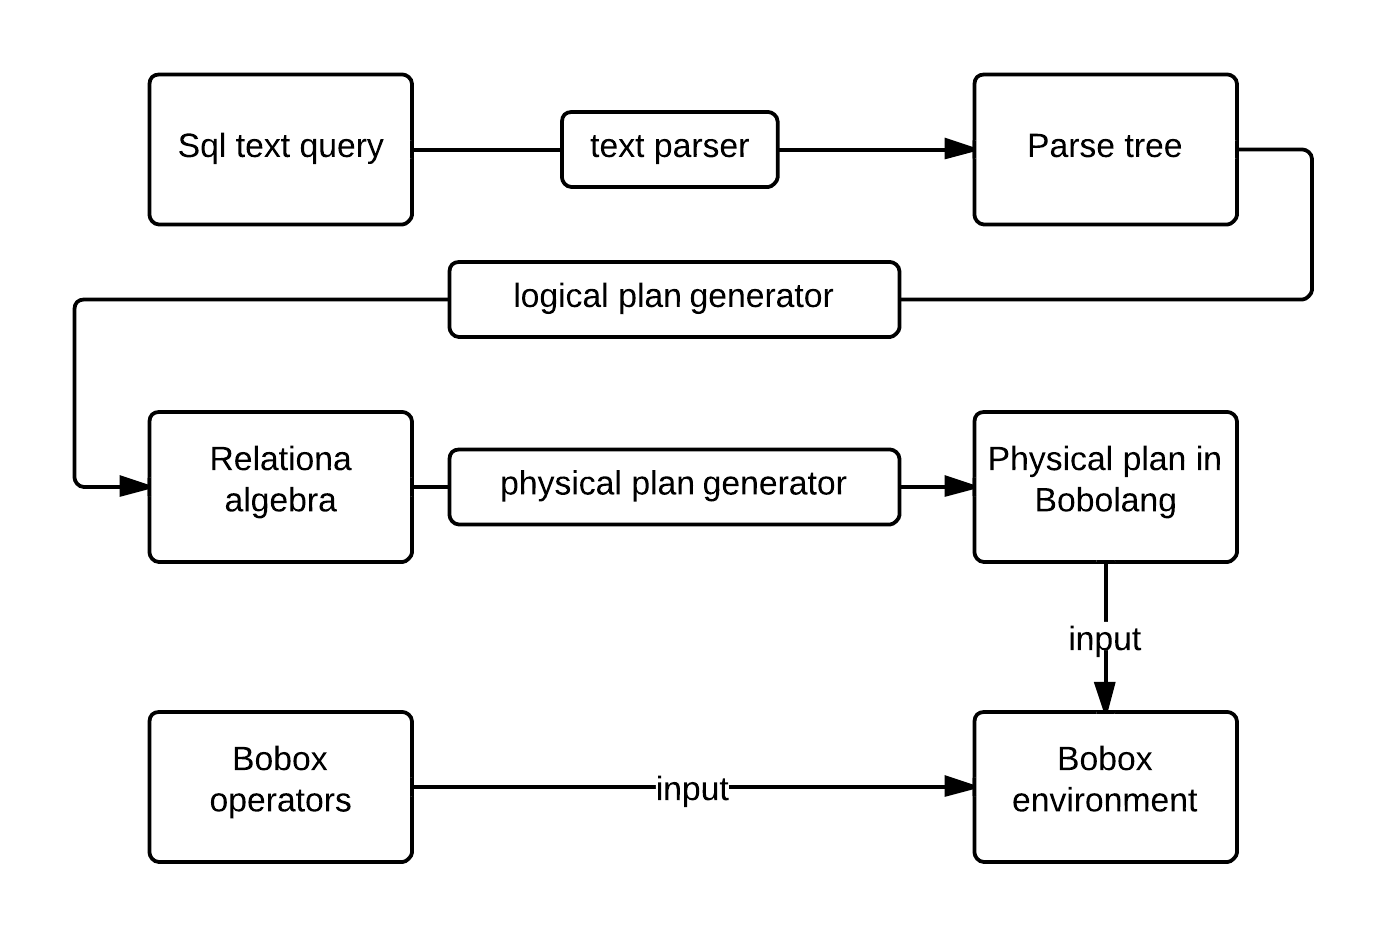
\includegraphics[width=1\textwidth]{sqlarchitecture}
    
      \caption{SQL compiler architecture.}
        \label{fig:sqlarchitecture}
\end{figure}
SQL query is written in text. This text is parsed into parse tree, which is transformed into logical query plan (Relational algebra). Relational algebra is then optimized and this form is used for generating physical query plan. Physical plan written in Bobolang is input for Bobox for execution. Physical plan is not enough, we need to provide implementation of physical algorithms (Bobox operators).

Since SQL is a pretty complicated language, this thesis aim is only implementing optimization and transformation of logical plan into physical plan. This part is displayed as physical plan generator in figure~\ref{fig:sqlarchitecture}.


The main goal of this thesis is to implement part of SQL compiler. The input is query written in XML format in from of relational algebra. Program reads input and builds relational algebra tree, which is then checked for semantic errors. Then we improve logical plan by pushing selection down the tree. From improved relational algebra tree we generate physical plan. In this phase we assign physical algorithm for every logical plan operator and we also choose order of joins. The output is execution plan for Bobox written in Bobolang.

\chapter{Architecture}

\section{Bobox}

In the section we describe basic architecture of Bobox. Information source for this chapter is Doctoral thesis\cite{faltthesis}. 

Overall Bobox architecture is displayed in figure~\ref{fig:bobox}. Framework contains of Boxes. Box is basically a C++ class containing implementation of data processing algorithm or it can be set of connected boxes. Box can have arbitrary number of inputs and outputs. All boxes are connected to a directed acyclic graph.  

\begin{figure}[h!]
  \centering
    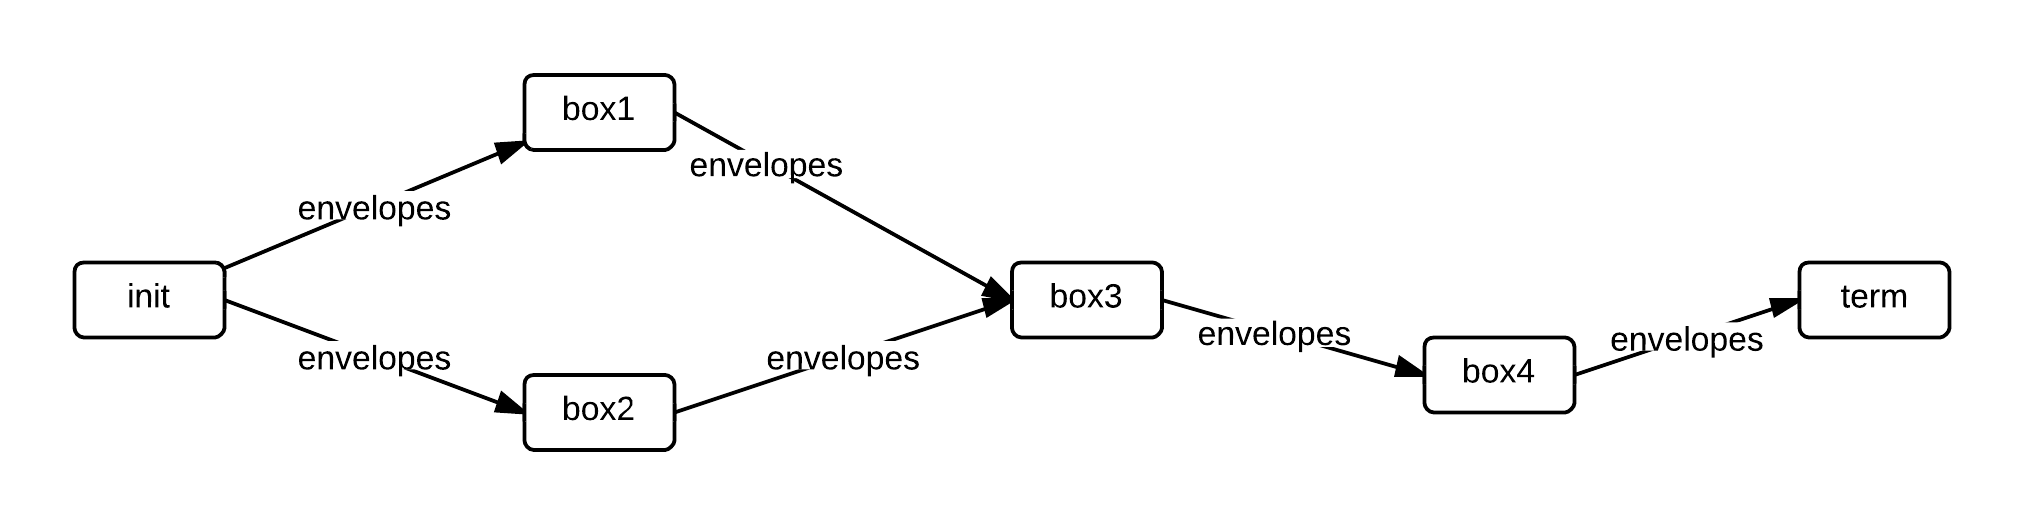
\includegraphics[width=1\textwidth]{bobox}

      \caption{Bobox architecture.}
          \label{fig:bobox}
\end{figure}

Data streams are implemented as streams of data units called envelopes. Envelope structure is displayed in figure~\ref{fig:envelope}. It consists of sequence tuples, but internally data are stored by columns, that means envelope contains from sequence of columns and it's data is stored in separate list. So to read all attributes of the i-th tuple we have to access all column lists and read it's i-th element. There is special type of envelope having poisoned pill. It is send after all valid data indicating end of data stream. 

\begin{figure}[h!]
  \centering
    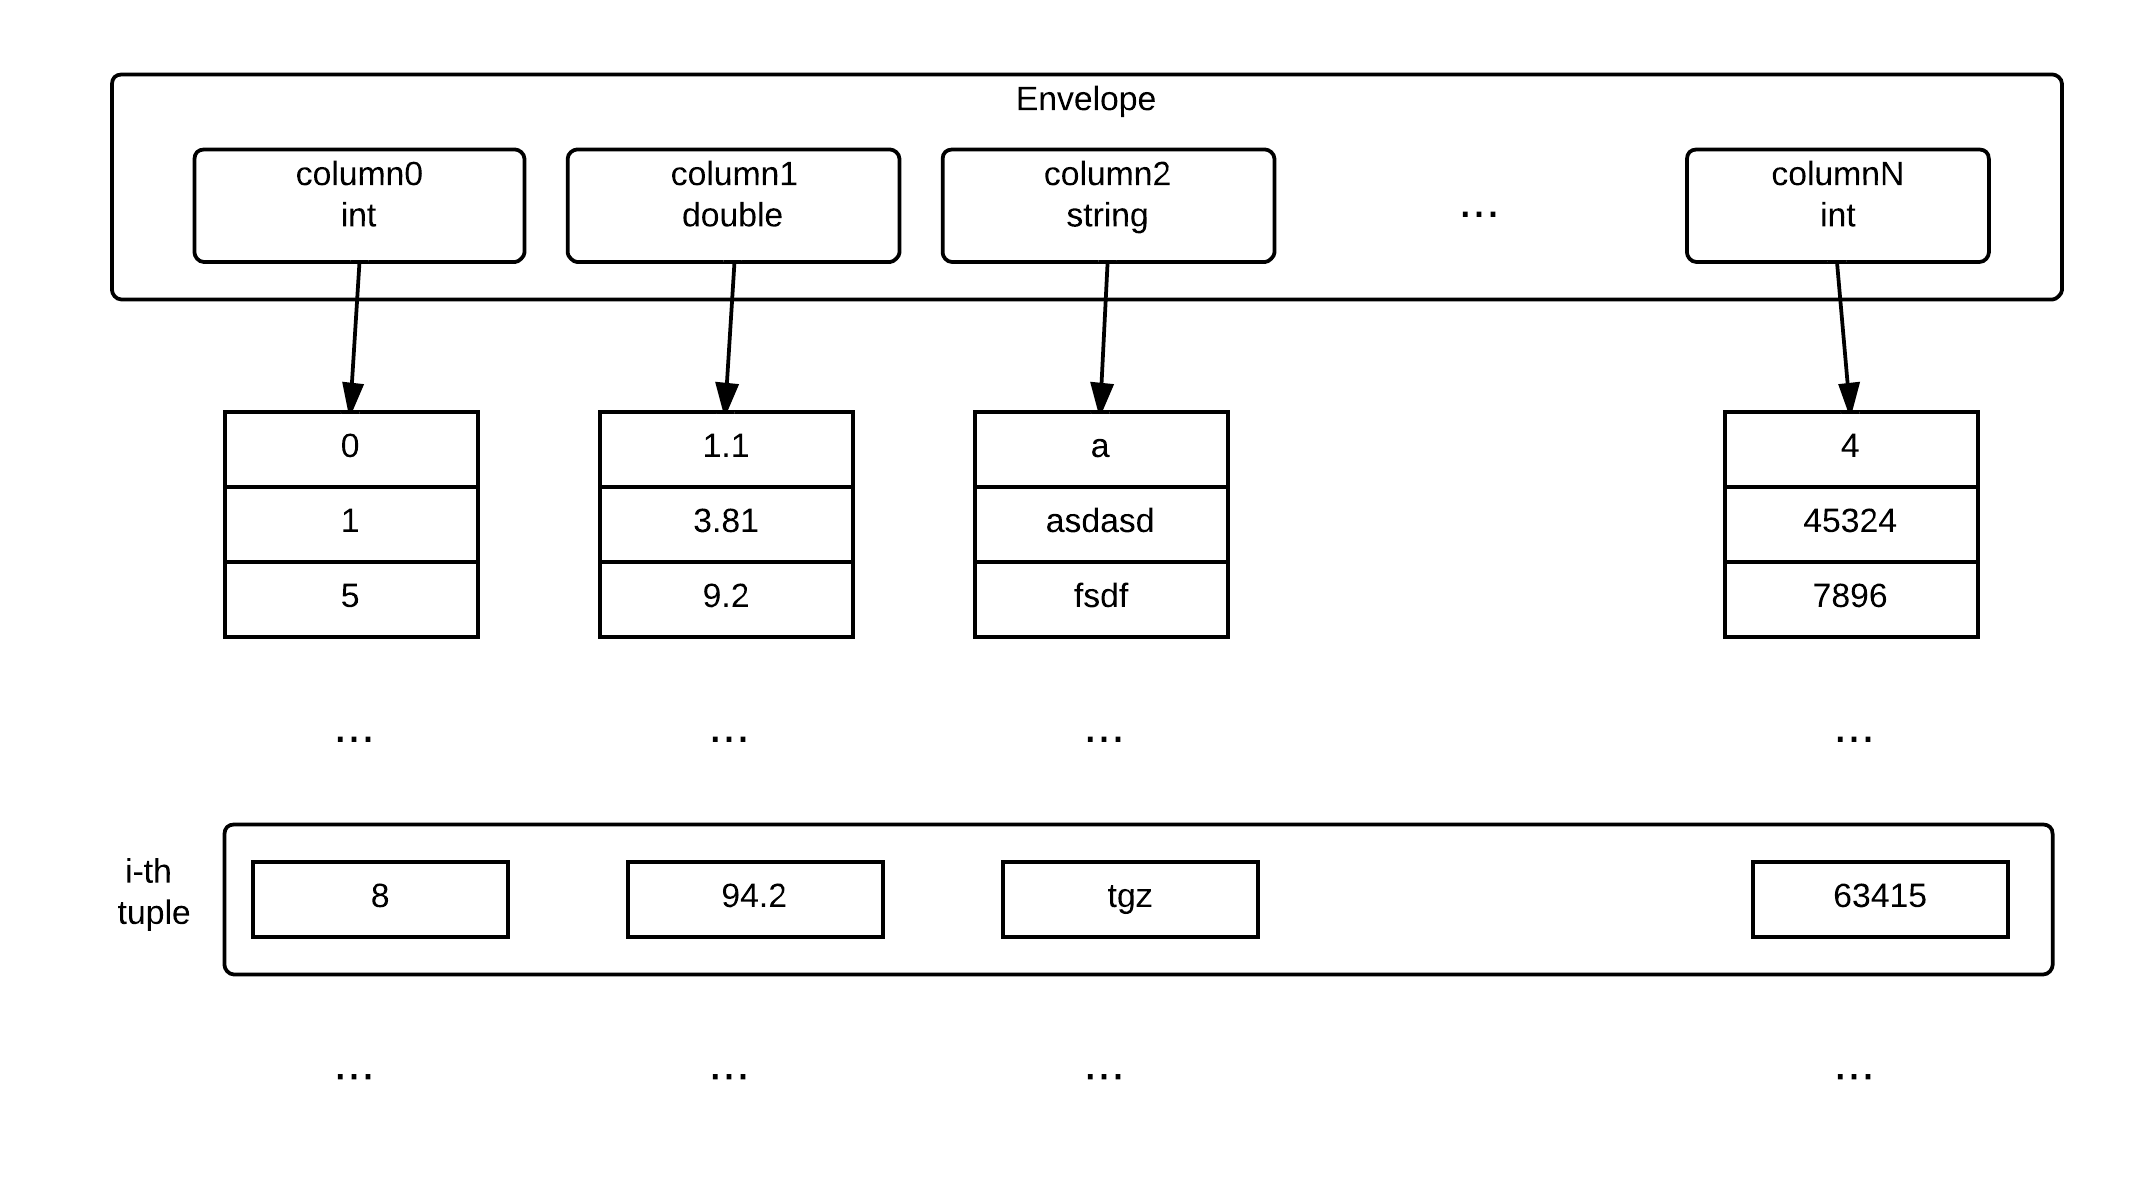
\includegraphics[width=1\textwidth]{envelope}

      \caption{Envelope structure.}
          \label{fig:envelope}
\end{figure}
There are two special boxes, which have to be in every execution plan:
\begin{itemize}


\item $init$ - first box in topological order and it indicates starting box of execution plan

\item $term$ - last box in topological order and indicates that plan has been completely evaluated

\end{itemize}

Evaluation starts with scheduling $init$ box, which sends poisoned pills to all of its output. All of it's output boxes will be scheduled. They can read data from hard drive or network, process it and sent it to other boxes for further processing. Other boxes usually receives data in envelopes in their inputs. Box $term$ waits for every it's input to receive poisoned pill and then evaluation ends.

\section{Bobolang}
In this section we describe syntax and semantics of Bololang language. We used paper\cite{bobolang} as information source.

Bobolang is a formal description language for Bobox execution plan. Bobox environment provides implementation of basic operators (boxes). Bobolang let's programmer choose which boxes to used, what boxes to use, what type are passed and how the boxes are interconnected. 

We can define whole execution plan using operator main with empty input and output. Example of whole Bobolang plan:

\begin{verbatim}
operator main()->()
{
    source()->(int) src;
    process(int)->(int,int,int) proc;
    sink(int,int,int)->() sink;

    input -> src -> proc; 
    proc -> sink;
    sink -> output;
}
\end{verbatim}

In the first part we declare operators, define type of input and output. For every declared operator we provide identifier. Second part specifies connection between declared operators. Code \verb|op1 -> op2| indicates that output of \verb|op1| is connected to input of operator \verb|op2|. In this case output type of \verb|op1| has equal to input type of \verb|op2|. Bobolang syntax also allows to create chains of operators like \verb|op1 -> op3| which has semantics like \verb|op1 -> op2| and \verb|op2 -> op3|. 

There are explicitly defined operators called \verb|input| and \verb|output|. They represents input and output of declared operator \verb|process|. The line \verb|input -> srce;| represents that input of the operator \verb|process| is connected to output of operator \verb|pre|.

Boblang also allows to declare operators with empty input or output. They have type \verb|()| that means it doesn't transfer any data. Only data allowed is to transfer poisoned pill. When box receives poisoned pill, it means that it should start working, Sending it means that it's work is done.


 In figure~\ref{fig:exampleplan} we can seen structure of example execution plan. Operators \verb|init| and \verb|term| are added automatically. Operator \verb|init| sends poisoned pill to \verb|source|, which can read data from hard drive or network. These data are send to box \verb|process|. Operator sink stores data and sends poisoned pill to box \verb|term| and the computation ends.
\begin{figure}[h!]
  \centering

    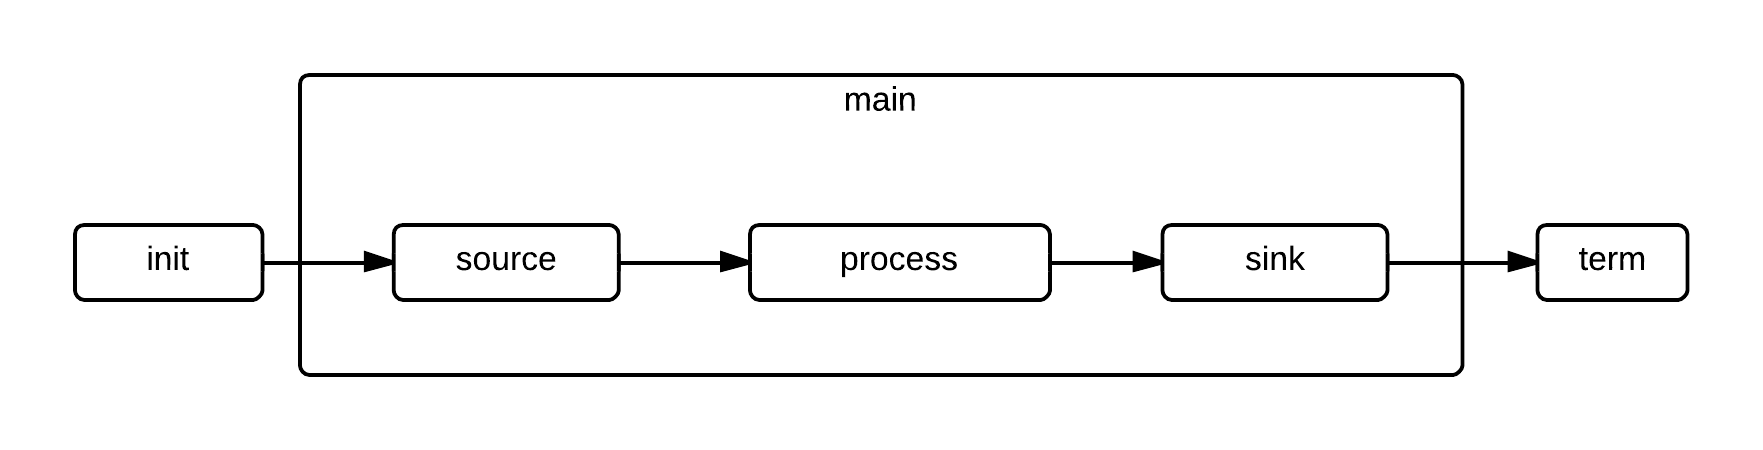
\includegraphics[width=1\textwidth]{exampleplan}
    
      \caption{Example of execution plan.}
        \label{fig:exampleplan}
\end{figure}





\chapter{Title of the second chapter}

\section{Title of the first subchapter of the second chapter}

\section{Title of the second subchapter of the second chapter}

\chapter{Analysis}

\section{Format of relational algebra}

In this section we present relation algebra operators which are used as input of compiler:
\begin{enumerate}
\item Projection - we used extended projection $\phi_L$, which remove columns, compute new columns using expressions and rename columns

\item Table operator, which is leaf or algebra tree. For this operator we need to provide arguments like:
\begin{itemize}
\item table name
\item information about index, like name and columns
\item columns to read
\end{itemize}
\item Join - we used theta join $\Join_C$. Condition $C$ can be in following format:
\begin{itemize}
\item Empty and in this case join represent Cartesian product.
\item $a_1=b_1~and~a_2=b_2~and~a_3=b_3~and...and~a_n=b_n$, where $a_k$ belong to first relation and $b_k$ belongs to other relation.
\item $a_1\oplus b \ominus a_2$, where $a_1$ and $a_2$ belong one input and $b$ belongs to second input. $\oplus$ and $\ominus$ can be $<$ or $\leq$.

\end{itemize}

In addition to condition we need to specify output attributes of join. They can be from both input and we can optionally assign them new name, in case we need to work with two attributes but they have same name.

Other types or joins are not directly supported, but can be replace with cross join with following selection.
\item Anti join wasn't presented with other join algorithms. We denote it $\ltimes_C$ where $C$ is anti join condition. Output of expression $R \ltimes_C S$ is relation with tuples from $R$, for which doesn't exist any tuple is $S$ that satisfy condition. We can us join and anti join to express outer join:
\begin{itemize}
\item 
 $R\Join^\circ_C S= (R\Join_C S)\cup (R\ltimes_C S)$
\end{itemize}
To be precise we need to add columns contain $null$ to result of anti join.
 
Other use is to compute difference $R-S$. This can be rewritten as $R \ltimes_C S$, where $C$ equates attributes from $R$ with same called attributes in $S$. 
 
Advantages of using this attribute is, that we don't need outer join and difference, which will make working with algebra a little easier.

In implemented tool condition $C$ of anti join can be in following format:
\begin{itemize}
\item $a_1=b_1~and~a_2=b_2~and~a_3=b_3~and...and~a_n=b_n$, where $a_k$ belong to first relation and $b_k$ belongs to other relation.
\end{itemize}
In addition to that, we also need to specify output attributes of anti join and optionally assign them a new name. They can be only from first input relation.
\item Group operator $\gamma_L$, where L is non empty list of group attributes and aggregate functions. Supported aggregate functions are $min$, $max$, $sum$ and $count$. Function $avg$ is not supported but it can easily computed. All mentioned functions except $count$ take one attribute as input, function count has empty input. 

As we mentioned before, group operator is more general version of duplicate elimination. That's why we don't include duplicate elimination in our algebra.
\item Sort operator $\tau_L$, where $L$ is a non empty list of attributes with sort directions.
\item Union - $\cup$ is set union. In case we want to bag union we can compute set union and eliminate duplicate using grouping operator. Requirement is that both relations have same number of columns and they have same name.
\item Selection - we used selection as described in classic relational algebra.

\end{enumerate}

\section{Physical algorithms}

In this section we enumerate and describe algorithms which are generated to output. We assume that queries have enough memory and physical operators doesn't have to store intermediate result on hard drive.

Here is a list on algorithms:
\begin{itemize}
\item $Filter$ - this algorithm reads input tuples and outputs tuple satisfying given condition. Output doesn't have to be sorted same way as input.
\item $Filter$ keeping order - this algorithm reads input tuples and outputs tuple satisfying given condition. Output has to be sorted same way as input.
\item $Hash~group$ - operator group tuples and computes aggregate functions. Grouping is performed using hash table.
\item $Sorted~group$ - operator groups tuples and computes aggregate functions. Input has to be sorted by group attributes.
\item $Column~operations$ - this is an implementation of extended projection algebra node. 
\item $Cross~join$ - this operator computes product of two relations.
\item $Hash~join$ - computes join with equal conditions using hash table. 
\item $Merge~equijoin$ - this algorithm computes join with equal conditions. Input relations has to be sorted by join attributes. Algorithm creates join result merging sorted relations.
\item $Merge~non~equijoin$ - operator computes theta join with condition $a_1\oplus b \ominus a_2$, where $a_1$ and $a_2$ belong one input and $b$ belongs to second input. Signs $\oplus$ and $\ominus$ can be $<$ or $\leq$. Input relations has to be sorted by join attributes. Algorithm computes join merging relations.
\item $Hash~anti~join$ -  algorithm computes anti join with equal conditions of two relations using hash table.
\item $Merge~anti~join$ - algorithm computes anti join with equal conditions. Input relations has to be sorted by join attributes.
\item $Table~scan$ - operator scans whole table from hard drive.
\item $Scan~and~sort~by~index$ - operator scans whole table from hard drive using index. Output will be sorted by columns on given index.
\item $Index~Scan$ - this algorithm uses index to read only tuples satisfying given condition.
\item $Sort$ - this algorithm sorts input. Input can be presorted, in this case operator uses this information and sorts only by not yet sorted attributes.
\item $Union$ - this operator is bag union, it only append tuples from one relation to another.

\end{itemize}

Nested loop joins are not supported, because it's implementation in Bobox can create cycles.

\section{Architecture}
The architecture of implemented tool is displayed in figure~\ref{fig:compilerarchitecture}.

\begin{figure}[h!]
  \centering
    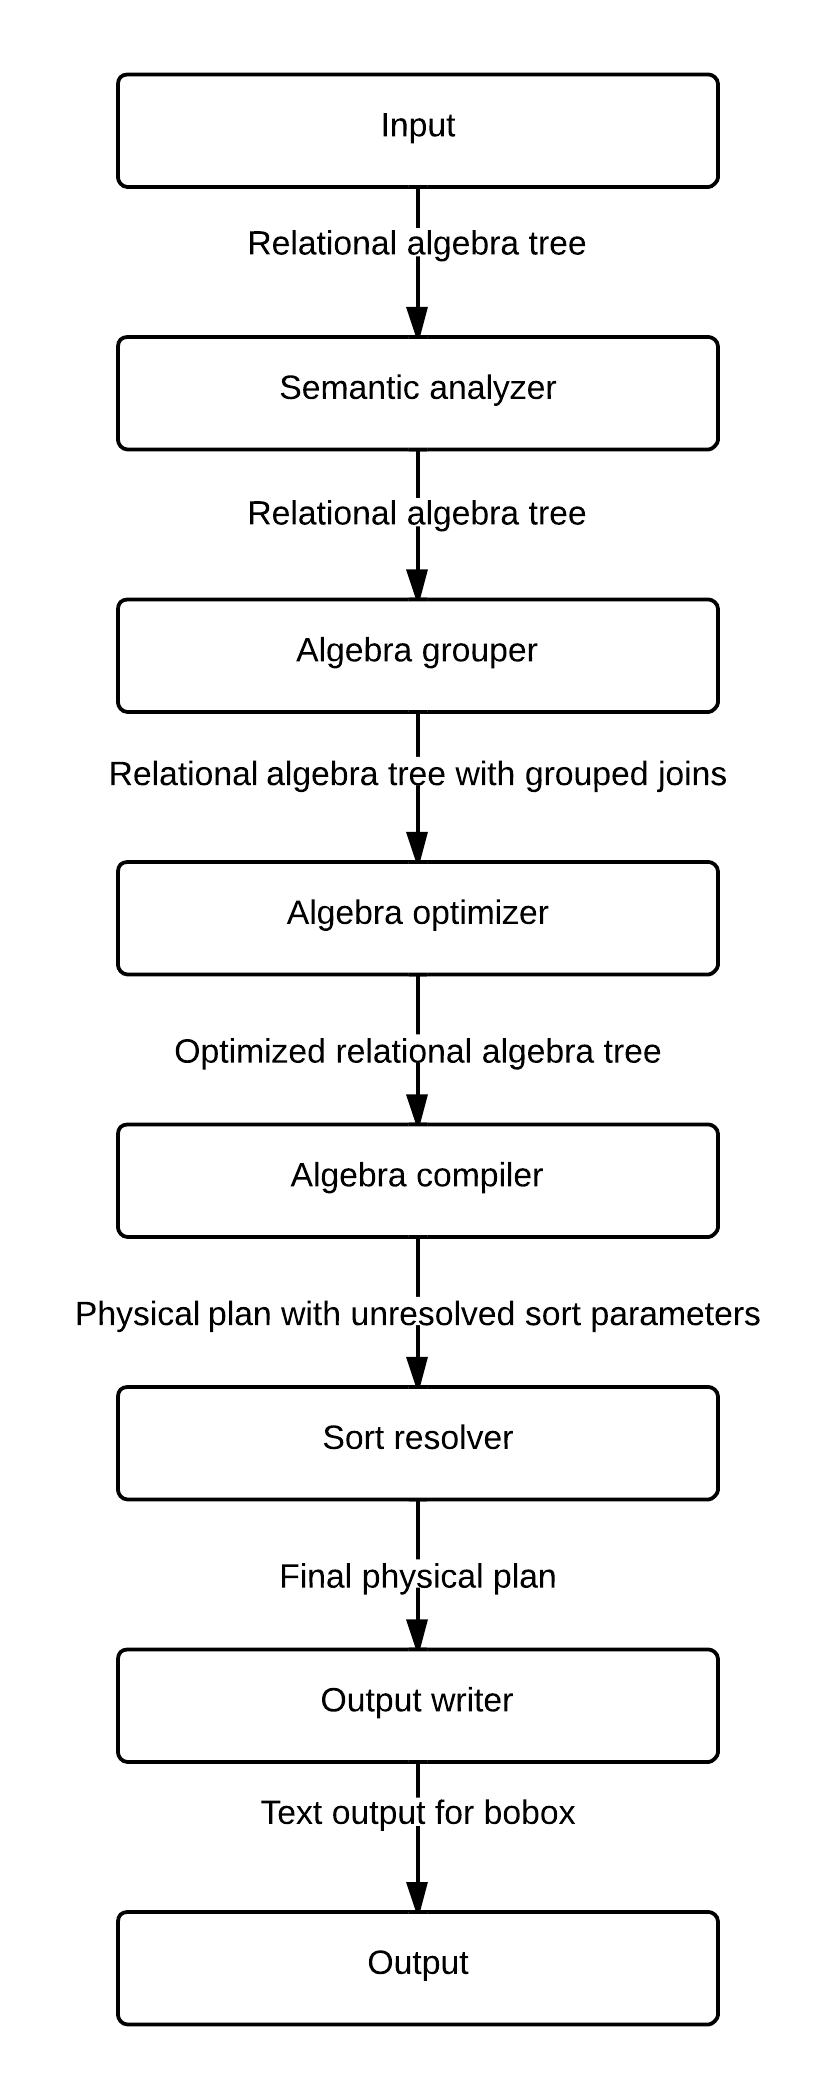
\includegraphics[width=0.5\textwidth]{compilerarchitecture}

      \caption{Compiler architecture.}
          \label{fig:compilerarchitecture}
\end{figure}

Relational algebra is read from input. the input is in XML format. For this format we decided for following reasons:
\begin{itemize}
\item XML has tree like structure exactly like relational algebra.
\item For validation we only need to write schema.
\item There are already implemented tools for parsing.
\item There is no need to write input parser.
\end{itemize}

After that relational algebra tree is checked in component called semantic checker. Semantic checker checks if all of used attributes are on input of operator or if there are no duplicate operators. 

Semantically correct tree goes to component that groups neighboring joins into one. This is done so we can choose fastest way to join multiple relations.

Algebra tree with grouped joins is optimized. We implemented one most important optimizations pushing selections down the tree. This component also pushes selection to join if selection contains equal condition, where one argument is from first and second argument is from second input.

Optimized algebra tree is processed by compiler, which generates physical plan which. This plan is not final. It's sort operator's parameters doesn't have to be final. For example if we want to sort relation before grouping we can sort it in different directions and than later decide what direction is better.

Final plan is output of component named Sort resolver. This component decides unknown sort order of sort operators.

Final plan is then converted to Bobolang in Output writer.

Implemented tool doesn't check types. Since it will be back end of compiler, the assumption is that front end parsing text will handle types. Types are only copied to output and we assume that there are no mistakes in types.

\section{Data structures}

In this chapter we describe data structures used in implementing tool.

Relational algebra si stored in polymorphic tree. Every node stores it's parameters pointer on parent in the tree and zero or more pointer on children node. No other structure was considered for this representation since this is efficient way to store logical plan. It allows easily to add new types of relational algebra operators and it is not had to manipulate with the tree. We can remove or add new node very easily. 
Example of this representation can be found in figure \ref{fig:groupalgebra}. It's representing simple query reading whole table, then grouping it and computing some aggregation functions. The result is sorted at the end. Leaf of the tree also stores some information about indexes on read table, list of columns with their type and number of unique values. Other important parameter is size of relation which is displayed in number of rows parameter.

\begin{figure}[h!]
  \centering
    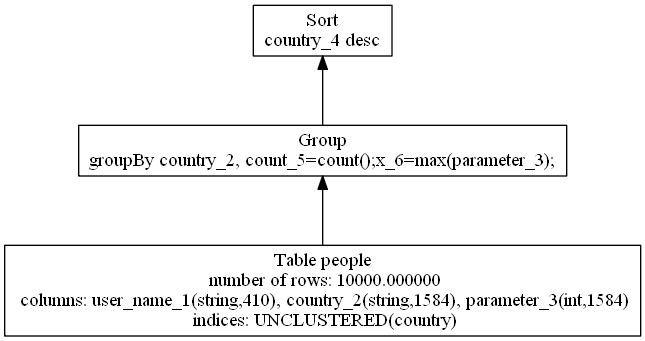
\includegraphics[width=0.8\textwidth]{groupalgebra}

      \caption{Example of relational algebra structure.}
          \label{fig:groupalgebra}
\end{figure}

We choose same structure for physical plan. Physical plan usually doesn't have to changes. The advantage of storing it into polymorphic tree is to ability to easily add new root node. Example of this representation can be found in figure \ref{fig:groupplan}. This figure contains one of possible physical plans for relational algebra in figure  \ref{fig:groupalgebra}. For reading we used algorithm table scan, then we hashed input by requested columns and at the end we sorted it using sort operator. Every nodes stores additional information like output attributes, estimated time it's going to need and size of output relation.

\begin{figure}[h!]
  \centering
    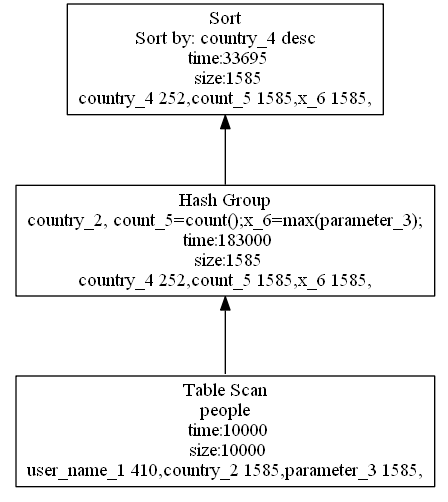
\includegraphics[width=0.6\textwidth]{groupplan}

      \caption{Example of physical plans structure}
          \label{fig:groupplan}
\end{figure}
More complicated structure was used to storing join parameters. This structure is stored in every sort physical operator to determine what columns should relation be sorted by. 

If we want to use group operator based on sort and it groups by three columns, we don't know which sort direction to use. Let's have expression $\gamma_{x,y}(R)$. There is four way to sort expression before calling group operator. This ways are:
\begin{itemize}
\item $x:A,y:A$
\item $x:A,y:D$
\item $x:D,y:A$
\item $x:D,y:D$
\end{itemize}
$A$ means ascending and $D$ is abbreviation for descending.

If we want to use merge join, joining on two attributes, we don't know direction and also which column should be first and which second. For example let's have $R\Join_{r_1=s_1~and~r_2=s_2} S$. In this case we can sort relation $R$ following way:
\begin{itemize}
\item $r_1,r_2$
\item $r_2,r_1$
\end{itemize}
Order, how to sort columns is also unknown.

We also want to store information about equality of sort column. After merge join $R\Join_{r_1=s_1} S$ is result sorted by $r_1$ or $s_1$.

All this requirements were use to design structure to store sort parameter without enumerating all possible sort orders.

\begin{figure}[h!]
  \centering
    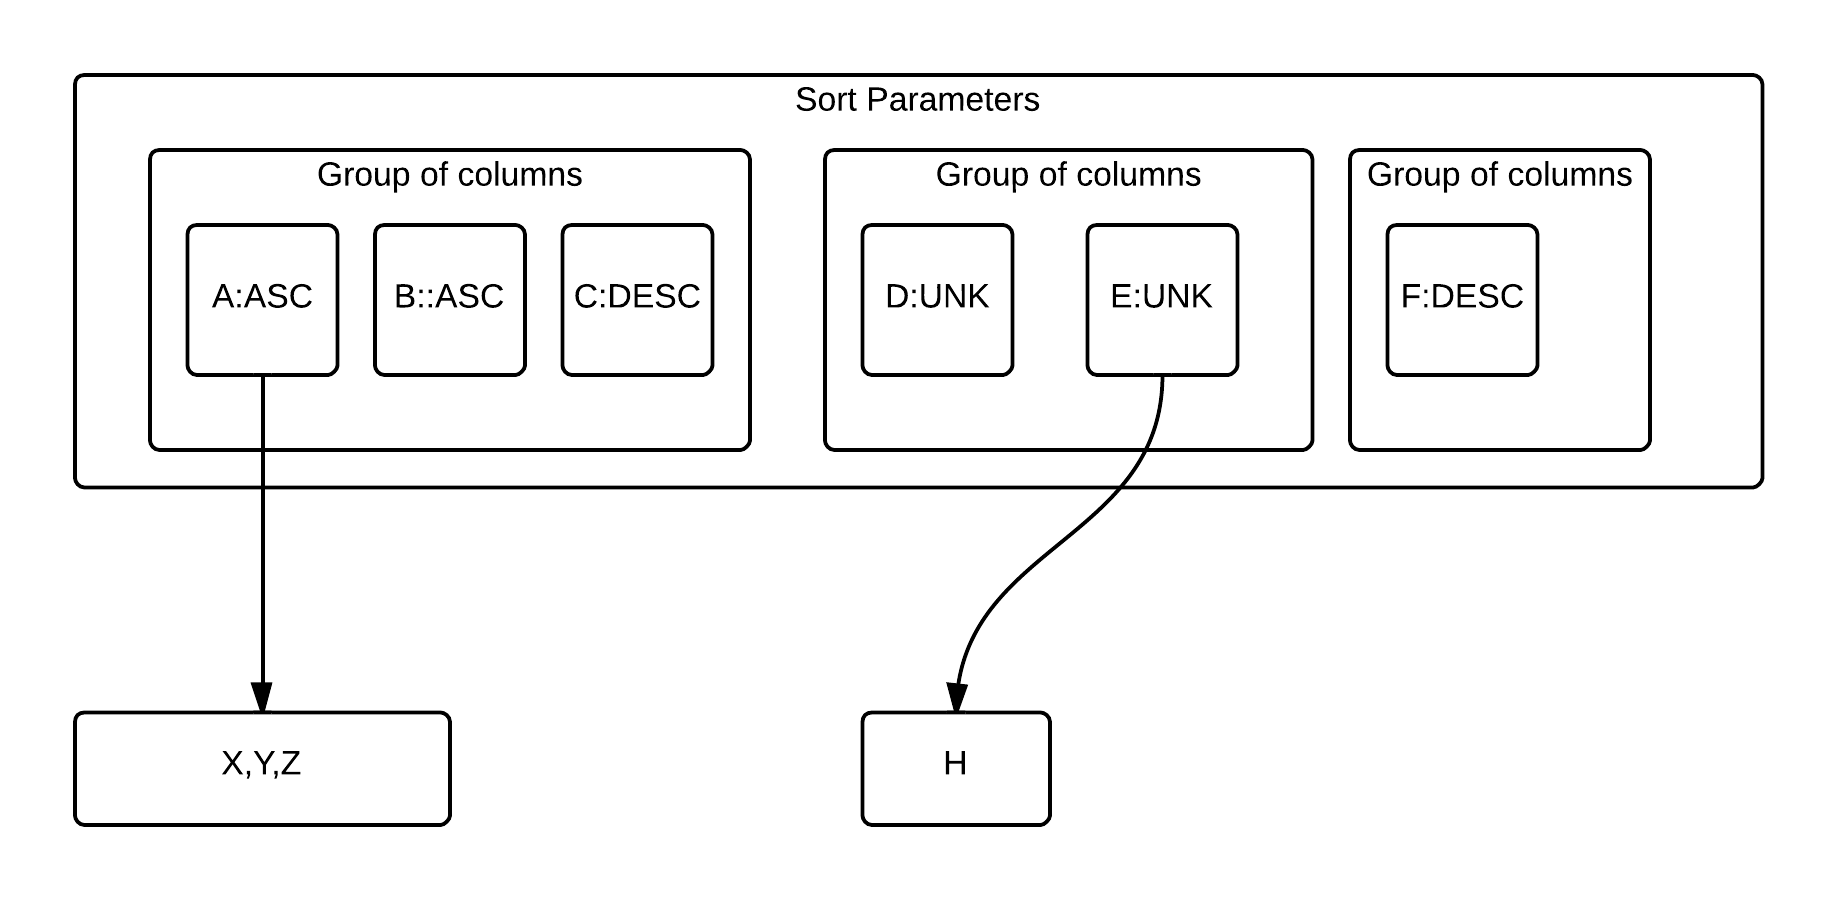
\includegraphics[width=0.9\textwidth]{sortparameters}

      \caption{Structure storing parameters for sort.}
          \label{fig:sortparameters}
\end{figure}

In figure \ref{fig:sortparameters} we display an example of sort parameters, which sorts by 6 columns. It usually contains from 1 or more columns group. The meaning is that order of columns groups is set. Order of columns in groups is arbitrary. It means that $F$ has to be on sixth place, but column $E$ can be on forth of fifth. Every column contains information about sort order: $ASC$ (ascending), $Desc$ (descending) or $UNK$ (unknown - can be ascending or descending). Every column also can be list of attributes which are equal to it. If we for example in projection remove attribute $A$, we still have attributes $X$, $Y$ and $Z$ which are equal to it, so one can take it's place.

Figure \ref{fig:sortparameters} represents many sort order possibilities we enumerate only some of then:
\begin{enumerate}
\item $A:ASC,C:DESC,B:ASC,H:DESC,D:ASC,F:DESC$
\item $C:DESC,B:ASC,Z:ASC,H:DESC,D:DESC,F:DESC$
\item $B:ASC,C:DESC,A:ASC,E:ASC,D:DESC,F:DESC$
\item $C:DESC,B:ASC,Y:ASC,D:ASC,H:ASC,F:DESC$
\end{enumerate}



\section{Optimization}

In this section we describe algebra optimization, which were implemented to improve logical plan.


\section{Generating physical plan}





\chapter{Implementation}
\label{implementation}
In this chapter we describe implementation details in the developed software and its functionality using examples. More implementation details can be found on the CD in generated doxygen\cite{doxygen} documentation. We will use following example to describe optimizations and plan generation:


\begin{verbatim}
select
    l_orderkey,
    sum(l_extendedprice*(1-l_discount)) as revenue,
    o_orderdate,
    o_shippriority
from
    customer,
    orders,
    lineitem
where
    c_mktsegment = '[SEGMENT]'
    and c_custkey = o_custkey
    and l_orderkey = o_orderkey
    and o_orderdate < date '[DATE]'
    and l_shipdate > date '[DATE]'
group by
    l_orderkey,
    o_orderdate,
    o_shippriority
order by
    revenue desc,
    o_orderdate;
\end{verbatim}

This example is taken from TPC benchmark\cite{benchmark}. $[DATE]$ and $[SEGMENT]$ are constants. Tables do not contain any indices in this benchmark. Columns starting with o\_ are from table order, columns beginning with l\_ are from table lineitem and columns with prefix c\_ belongs table customers.



\section{Input}

Input is XML file containing logical query plan. In this section we describe its structure. 

\subsection{Sort}

The root of every tree contain the sort operator, even if output does not have to be sorted. In this case sort has empty parameters.The following example displays sort operator structure:


\lstset{
  language=XML,
  morekeywords={encoding,
    xs:schema,xs:element,xs:complexType,xs:sequence,xs:attribute}
}
\begin{lstlisting}
<?xml version="1.0" encoding="utf-8"?>
<sort xmlns:xsi="http://www.w3.org/2001/XMLSchema-instance"
 xsi:noNamespaceSchemaLocation="algebra.xsd">
  <parameters>
    <parameter column="revenue" direction="desc" />
    <parameter column="o_orderdate" direction="asc" />
  </parameters>
  <input>
  ...
  <input>
</sort>
\end{lstlisting}

The sort is a root element of XML file. Inside the parameters there is specified how to sort relation. This example represents sort $\tau_{revenue:desc,o\_orderdate:asc}(...)$. The element $input$ should contain other algebra tree node.

\subsection{Group}

Next example displays the group node:

\begin{lstlisting}
<group>
  <parameters>
    <group_by column="l_orderkey"/>
    <group_by column="o_orderdate" />
    <group_by column="o_shippriority"/>
    <sum argument="x" output="revenue"/>
  </parameters>
  <input>
  ...
  <input>
</group>
\end{lstlisting}

This node represents expression $\gamma_{l\_orderkey,o\_orderdate,o\_shippriority,x=sum(x)}(...)$. Group element has to have at least one group by parameter or at least one aggregate function. Inside the element $input$ there should be an other operator.

\subsection{Selection}

The selection presented in the following example:

\begin{lstlisting}

<selection>
  <parameters>
    <condition>
      <lower>
        <constant type="date" value="today"/>
        <column name="l_shipdate"/>
      </lower>
    </condition>
  </parameters>
  <input>
  ...
  </input>
</selection>
\end{lstlisting}
This example represents following expression: $\sigma_{today<l\_shipdate}$. The condition element we can contain multiple conditions connected by $and$ or $or$ elements. Input algebra supports operators $=$,$<$ and $\leq$. In the leafs of expression tree there can be only column or constant element. We also can call a boolean function from selection and this call is presented in the following example:

\begin{lstlisting}
<condition>
  <boolean_predicate  name="like">
    <argument>
      <column name="x"/>
    </argument>
    <argument>
      <constant type="int" value="445" />
    </argument>
  </boolean_predicate>
</condition>
\end{lstlisting}

Using boolean predicate it has to be supported by runtime (Bobox operators). The compilee does not check if called predicate does exist.

\subsection{Join}

The join operator without condition represents cross join. We can use join with multiple equal conditions or with one simple unequal condition. The first example contains equal conditions:

\begin{lstlisting}
<join>
  <parameters>
    <equal_condition>
      <equals>
        <column name="a"/>
        <column name="b"/>
      </equals>
      <equals>
        <column name="c"/>
        <column name="d"/>
      </equals>
    </equal_condition>
    <column name="a" input="first"/>
    <column name="b" input="second"/>
    <column name="c" input="first"/>
    <column name="d" input="second" newName="e" />
  </parameters>
<input>
...
</input>
\end{lstlisting}

This example represents join with condition $a=b~and~c=d$. In join equal conditions of this join, first column has to be from the first relation and second column comes from the second relation. The columns $a$ and $c$ are from the first input and $b$ and $d$ are from the other one. Joins does not copy all columns to output. We have to specify non empty sequence of output columns. For every column we have to specify name and the input number. We can also rename join output column by using attribute $newName$. In last example we renamed output column $d$ to $e$.

Next example shows join with inequality condition:

\begin{lstlisting}
<join>
  <parameters>
    <less_condition>
      <and>
        <lower_or_equals>
          <column name="a1"/>
          <column name="b"/>
        </lower_or_equals>
      <lower_or_equals>
        <column name="b"/>
        <column name="a2"/>
      </lower_or_equals>
    </and>
  </less_condition>
  <column name="a1" input="first"/>
  <column name="b" input="second"/>
  <column name="a2" input="first"/>
</parameters>
<input>
...
</input>
</join>
\end{lstlisting}
This example represents join with condition $a1\leq b\leq a2$. First element $lower\_or\_equals$ has to contain the column from first relation followed by column from the second relation. On the other hand the second element $lower\_or\_equals$ needs to specify these columns in reversed order. The element $lower\_or\_equals$ can be replace by the element $lower$. The rules for specifying output column are the same like in the join with equal conditions. The element $input$ should contain two algebra operators.

\subsection{Anti join}

\begin{lstlisting}
<antijoin>
  <parameters>
    <equal_condition>
      <equals>
        <column name="d"/>
        <column name="b"/>
      </equals>
    </equal_condition>
    <column name="d"/>
  </parameters>
<input>
...
<input>
</antijoin>
\end{lstlisting}
This is an example of antijoin with simple condition $d=b$. The structure is almost the same like in the join. Output columns can be only from the first relation and we can rename these columns.

\subsection{Table}
Table operator is the leaf of the algebra tree. We specify here the name of read table, its columns and indexes in table operator. The number of rows can be given in order to get better plans. If we do not have that information, we assume that a table has 1000 tuples. For every column we have to specify its name and type. Other optional parameter is $number\_of\_unique\_values$. This number is important for estimating size of join. If this information is missing, we will assume, that $number\_of\_unique\_values$ is size of table to power of $\frac{4}{5}$. This assumption is only experimental, since the number of unique values is from interval $\langle 0, table~size\rangle$. There are two types of indices. clustered and  unclustered. Table can have only one clustered index. For every index, we have to specify attributes and sort order. The following example contain table algebra node:
 
\begin{lstlisting}
<table name="orders" numberOfRows="1500000">
  <column name="o_orderdate" type="int"/>
  <column name="o_shippriority" 
  type="int" number_of_unique_values="30000"/>
  <column name="o_orderkey" type="int"/>
  <column name="o_custkey" type="int" />
  <index type="clustered" name="index">
    <column name="o_orderdate" order="asc" />
    <column name="o_shippriority" order="asc" />
  </index>
</table>
\end{lstlisting}

\subsection{Union}
The union operator does not have any parameters but columns from both inputs have to have the same names, for example:
\begin{lstlisting}
<union>
  <input>
  ...
  </input>
</union>
\end{lstlisting}

\subsection{Extended projection}
Following example of extended projection represents expression \\ $\pi_{l\_orderkey,o\_orderdate,o\_shippriority,x=l\_extendedprice*(1-l\_discount)}(...)$:
\begin{lstlisting}
<column_operations>
  <parameters>
    <column name="l_orderkey"></column>
    <column name="o_orderdate"></column>
    <column name="o_shippriority"></column>
    <column name="x">
      <equals>
        <times>
          <column name="l_extendedprice"/>
          <minus>
            <constant type="double" value="1"/>
            <column name="l_discount"/>
          </minus>
        </times>
      </equals>
    </column>
  </parameters>
  <input>
  ...
  </input>
</column_operations>
\end{lstlisting}

The extended projection contains a list of columns. Newly computed columns contains element $equals$ with expression. Expression tree can contain arbitrary function call which has to be supported by Bobox operators. Following example displays function call:


\begin{lstlisting}
<column_operations>
  <parameters>
    <column name="x">
      <equals>
        <aritmetic_function name ="sqrt" returnType="double">
          <argument>
            <constant type="double" value="2"/>
          </argument>
        </aritmetic_function>
      </equals>
    </column>
  </parameters>
  <input>
    ...
  </input>
</column_operations>
\end{lstlisting}
 
 We computed new column named $x$ with values $\sqrt{2}$.
 
\section{Building relational algebra tree} 

In this section we describe in more details structure storing logical plan and its building. Relational algebra operators are represented by children of the abstract class \texttt{AlgebraNodeBase}. It has following abstract subclasses:
\begin{itemize}

\item \texttt{UnaryAlgebraNodeBase} - abstract class for algebra operator with one input.

\item \texttt{BinaryAlgebraNodeBase}  - abstract class for algebra operator with two inputs.

\item \texttt{GroupedAlgebraNode} - abstract class for algebra operator with variable number inputs.

\item \texttt{NullaryAlgebraNodeBase} -  abstract class for algebra tree leafs.

\end{itemize}

All algebra operators are children of one of the mentioned classes. Every operator has pointer to its parent in the tree and smart pointers to its children if it has any. 

Expressions in nodes are represented by polymorphic trees. All expression nodes are children of class \texttt{Expression}.

For manipulating and reading expression and algebra tree we used the visitor pattern. All nodes (algebra and expression) contains method \texttt{accept}. This method calls visitor method on class \texttt{AlgebraVisitor}/\texttt{ExpressionVisitor}. All classes, which manipulate algebra tree, are children then of class \texttt{AlgebraVisitor}.


\begin{figure}[h!]
  \centering
    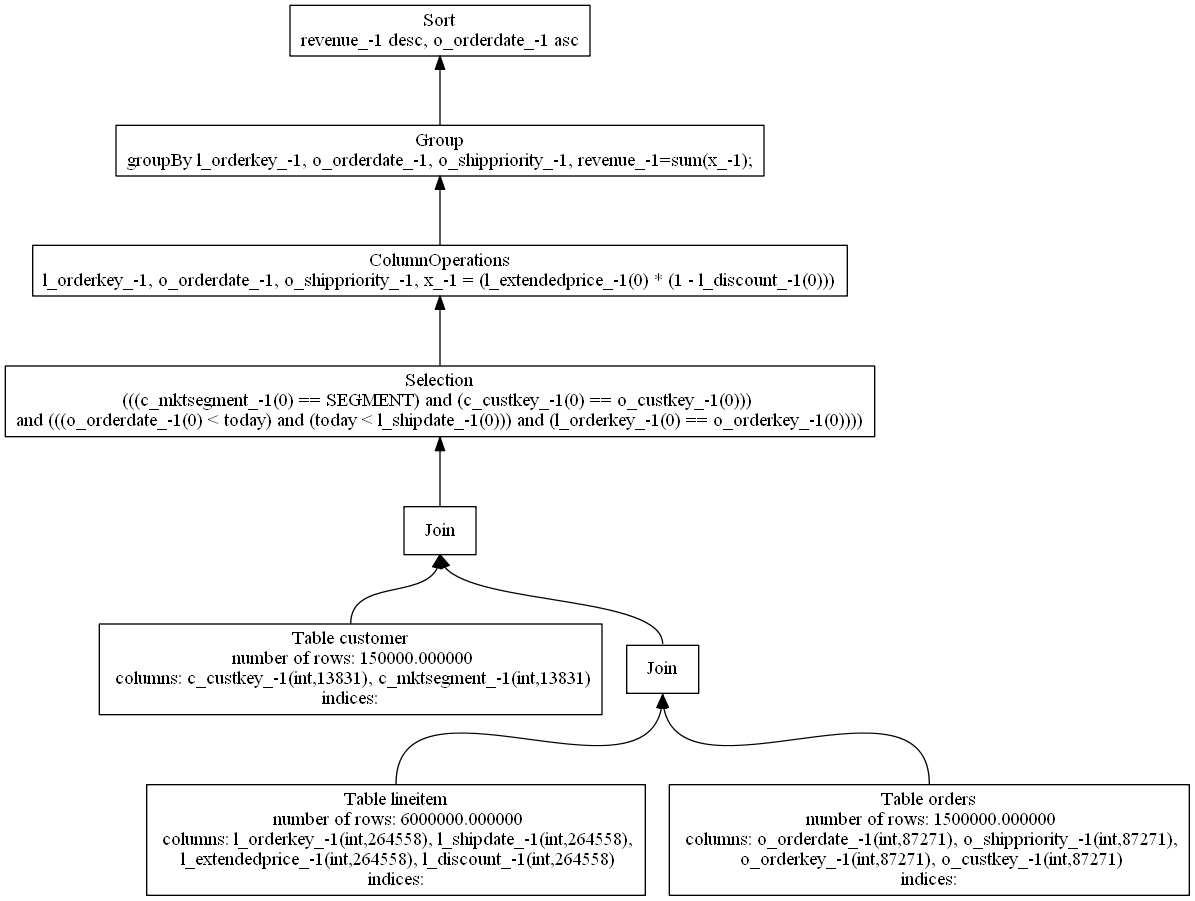
\includegraphics[width=1.0\textwidth]{algebratree1}

      \caption{Example of algebra tree.}
          \label{fig:algebratree1}
\end{figure}

In figure~\ref{fig:algebratree1} we presented the example of algebra tree of the query presented in the beginning of this chapter. We have transformed it to cross joins of three tables. After cross joins we applied selection with condition located in where clause. From the result we compute new column and apply grouping operator computing aggregate functions. Output of the query is sorted. In table reading operator we can see additional informations like name of table. Every attribute has the sufix $\_-1$ which is column's unique identifier. After the algebra tree is build from XML, unique identifiers are not assigned yet and they contain default value $-1$. The columns used in expressions contains number in parenthesis, which stores information which input does it belongs. Input operators are numbered from $0$. All columns used selection come from the $0^th$ input.

For parsing and validating input XML file we used library Xerces version 3.1.1~\cite{xerces}. It parses input file and creates DOM tree. This tree has to be validated against XML schema. Parsing and validation of XML is performed in the class \texttt{XmlHandler}.

Every algebra tree has to have sort operator on the top. We call \texttt{Sort} constructor with root element as an argument. This method copies all information from DOM tree and calls method \texttt{AlgebraNodeBase::constructChildren}, which decides what constructor to call on current node's children. This way we recursively build algebra tree.



\section{Semantic analysis and node grouping}

Semantic checking is processed by the class \texttt{SemanticChecker}, which checks if columns used in expression exist and if the output columns of operator have unique name. During this checking we assign unique identifier to every column. After this phase we do not need attribute names we use only the unique identifier.

Logical plan is after that visited by \texttt{GroupingVisitor}. In this phase are replaced joins represented by class \texttt{Join} by grouped join with two or more input relations. This node is represented by class \texttt{GroupedJoin}. For every expression we apply \texttt{GroupingExpressionVisitor}, which groups expressions with $and$ and $or$ operators. This step simplifies splitting condition into sub conditions.

\section{Algebra optimization}

We need to prepare logical tree for optimizing it by pushing down selections. To do this we split selection into smaller conditions using rule:
\begin{itemize}
\item $\sigma_{A~and~B}(R)=\sigma_{A}(\sigma_{B}(R))$
\end{itemize}
From every selection we created chain of selections. This operation is done by \texttt{SelectionSpitingVisitor}.

After that we call \texttt{SelectionColectingVisitor}. This visitor stores pointer of all selection in relational algebra tree. This pointers are input into \texttt{Push\-Selection\-Down\-Visitor}. It pushes all selections down the tree as much as possible and also converts cross joins into regular joins if we have selection with equal condition.
\begin{figure}[h!]
  \centering
    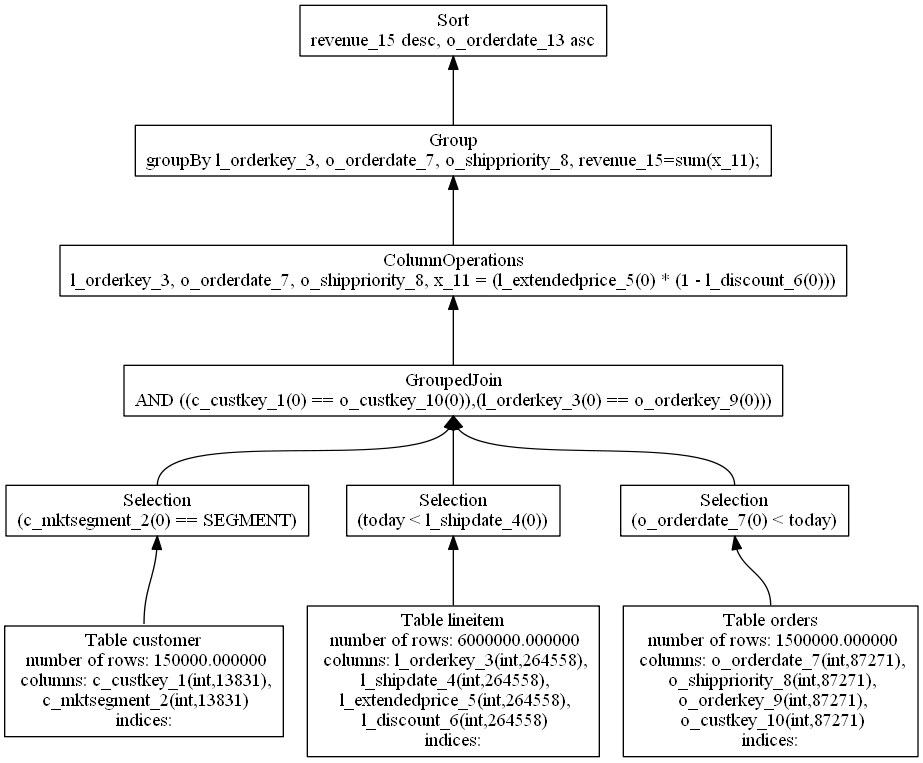
\includegraphics[width=1.0\textwidth]{algebratree2}

      \caption{Example of optimized algebra tree.}
          \label{fig:algebratree2}
\end{figure}
At this moment we have optimized tree, but we can find selection chains in it. To resolve this problem we apply \texttt{SelectionFusingVisitor}. This visitor applies following rule to tree:
\begin{itemize}
\item $\sigma_{A}(\sigma_{B}(R))=\sigma_{A~and~B}(R)$
\end{itemize}

In figure~\ref{fig:algebratree2} we can see optimizes algebra tree. In comparison figure~\ref{fig:algebratree1}, this tree has grouped join with three input relations. Also big selection about joins has been split and moved down the tree. Some part of condition became join condition other were pushed down on of branches of grouped join. Then we can see that new tree has columns with assigned unique identifiers. Because we have this identifiers we don't need to know number of input for each column.

This output is optimized algebra tree. We can of course implement more optimizations to improve logical plan.

\section{Generating plan}

Final logical plan will be processed by \texttt{AlgebraCompiler}, which outputs $n$ best plans. $n$ is a constant in  \texttt{AlgebraCompiler} represented by variable \texttt{NUM\-BER\_\-OF\_\-PLANS}. 

This visitor visits node of algebra tree, the it calls itself on its children. We use generated plans for child nodes to create plans for current node. After that we store best plans in variable \texttt{result}, relation size in variable \texttt{size} and output columns in variable \texttt{outputColumns}. 

For every node we generate all possible algorithms. Generated plans are stored in variable \texttt{result}. This variables stored a max-heap, where plans are compared by their overall time complexity. This time complexity is computed as sum of time complexity in all physical operators in current plan. This heap has maximal size of $n$. If there are more than $n$ plans we remove plan in root of the heap.

Both join order algorithms can be found in method \texttt{visitGroupedJoin}. If number of join relations is smaller than $k$ we used dynamic programing algorithm to estimate order of join. If we have more relations to join we use greedy algorithm. Constant $k$ is represented in variable \texttt{LI\-MIT\_\-FOR\_\-GREEDY\_\-JOIN\_\-ORDER\_\-ALGORITHM}. Both join algorithm call method \texttt{join}. This method combines plans and generates all possible plans.


Physical plan is represented as polymorphic tree. 


\begin{figure}[h!]
  \centering
    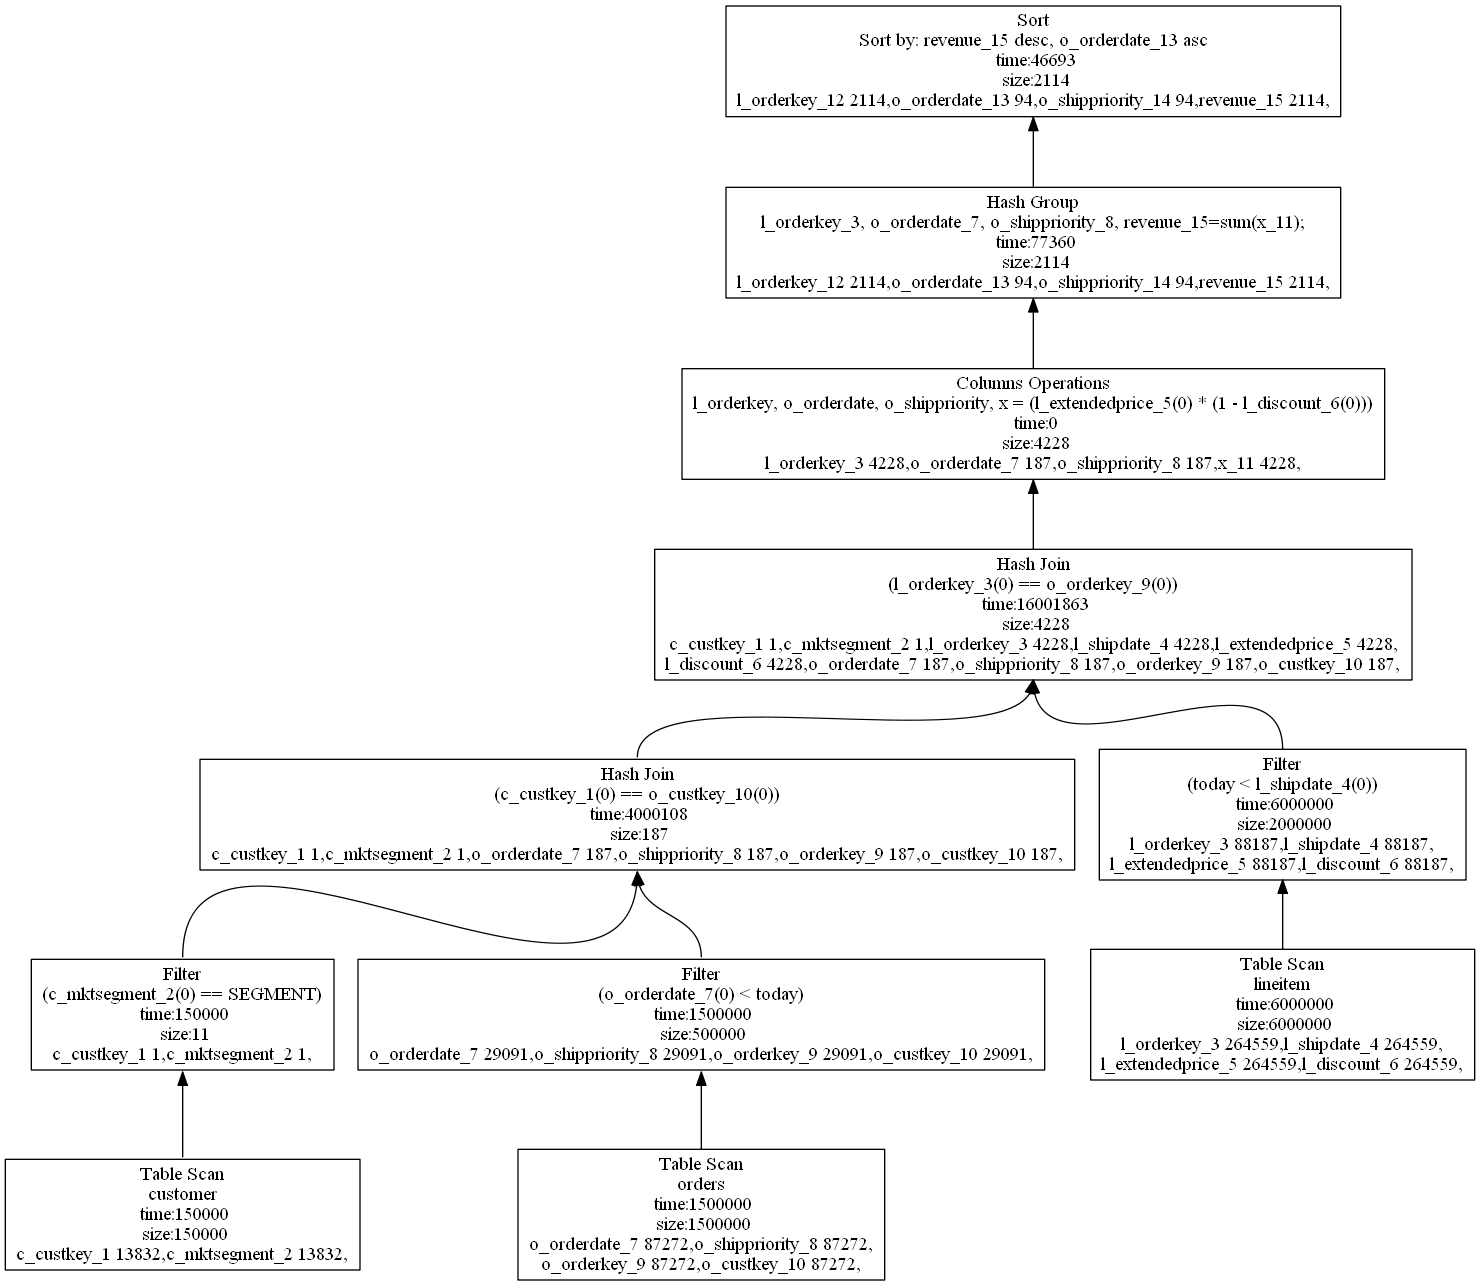
\includegraphics[width=1.0\textwidth]{physicalplan}

      \caption{Example of physical plan.}
          \label{fig:physicalplan}
\end{figure}


In figure \ref{fig:physicalplan} we can see best generated physical plan for query presented on the beginning of this chapter. Every operator contains estimated size and time. Below that we can see output columns with their unique identifiers and estimated number of unique values for each column. Since read tables doesn't contain any indexes, we have to read all the tables and filter results. After that we can only use hash join, because sorting relations for merge join would be to expressive and nested loop join is not supported by runtime or compiler. From the result we compute new columns and use hash group algorithm. We didn't use sorted group, because input is not sorted and output has to be sorted by other than group column.

Physical operators are chosen based on their estimated time complexity. It is computed from estimated size. In class \texttt{TimeComplexity} we have static functions which compute time complexity for each operation. It also contains constants used in this functions. We assume, that this constants or whole functions need to be improved. This improvement can be done base on testing and measuring evaluation queries in Bobox. At the time of submitting thesis runtime environment is not fully functional.




\section{Resolving sort parameters}

Sort parameters structure~\ref{fig:sortparameters} is represented by class \texttt{PossibleSortParameters}. Every columns group is stored in class \texttt{SortParameters}. Class \texttt{SortParameter} is used to store column name, sort direction.


We take generated plans from class \texttt{AlgebraCompiler}. Sort parameters of sort nodes need to be resolved. Two plans also can contain same physical operator. That's why need to clone plans, to assure that no algorithm representing object are used in two or more plans.

For cloning we used \texttt{CloningPhysicalOperatorVisitor}. Than we resolve generated plans in \texttt{SortResolvingPhysicalOperatorVisitor}. In figure~\ref{fig:plansortunresolved} we can see physical plan with unresolved sort parameters. 

\begin{figure}[h!]
  \centering
    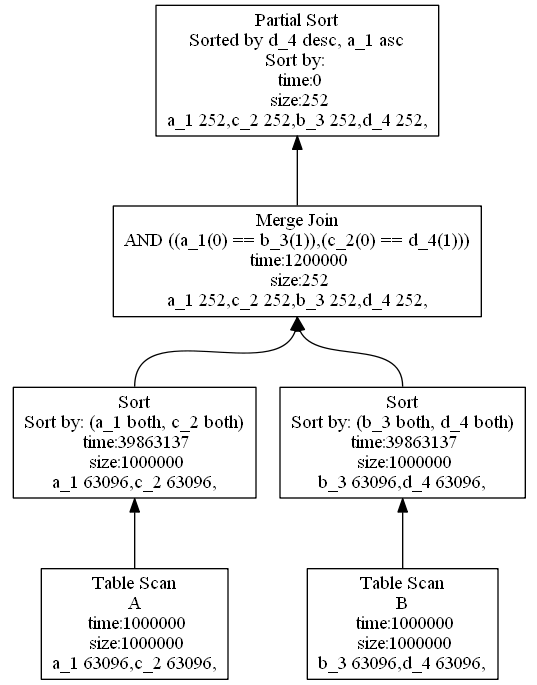
\includegraphics[width=0.6\textwidth]{plansortunresolved}

      \caption{Example of physical plan.}
          \label{fig:plansortunresolved}
\end{figure}

It contains two sort algorithms. Left one has following possible parameters:

\begin{itemize}
\item $a:both, c:both$
\item $c:both, a:both$
\end{itemize}

Right sort algorithm has sort parameters:
\begin{itemize}
\item $b:both, d:both$
\item $d:both, b:both$
\end{itemize}

At the time of generating this algorithm, we didn't know that order was the best to choose. After merge join plan has to be sorted by $d:desc,a:asc$. At the top of the tree we generated partial sort. It doesn't do anything because relation is already sorted. It only indicates, that from all sort parameter possibilities we chose $d:desc,a:asc$ and we don't have to do any additional sorting.

\texttt{SortResolvingPhysicalOperatorVisitor} works down tree. It uses variable \texttt{sortParameters}. We store there information how the input has been sorted before input of visited node. Using this variable we adjust sort parameters of sort algorithm. Adjusted plan is in figure~\ref{fig:plansortresolved}.

\begin{figure}[h!]
  \centering
    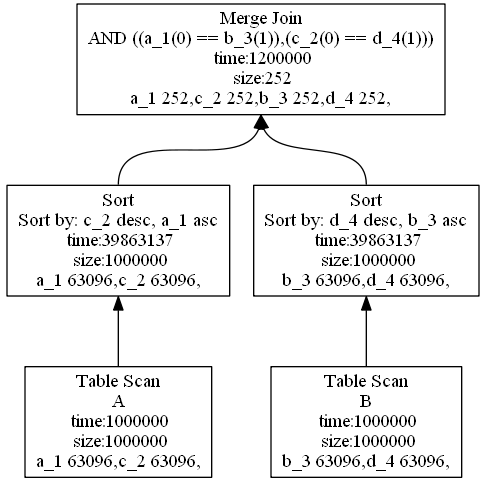
\includegraphics[width=0.6\textwidth]{plansortresolved}

      \caption{Example of final physical plan.}
          \label{fig:plansortresolved}
\end{figure}

Output od the query has to be sorted by $d:desc,a:asc$. Visitor sets that input of partial sort has to be sorted by $d:desc,a:asc$. After that we resolve in merge join that left input has to be sorted by and right input has to be sorted by $c:desc,a:asc$ $d:desc,b:asc$. Using this information we choose correct sort parameters in sort algorithms. 

There can be situations where we use sort based algorithm but output doesn't been sorted, we can choose arbitrary order of sort parameters. 


\section{Output}

 Output in Bobolang is generated by \texttt{BoboxPlanWritingPhysicalOperatorVisitor}. We can also generate output from algebra tree. Visitor \texttt{GraphDrawingVisitor} can generate output in dot language. Physical plan's output can be generated in dot language using \texttt{Physical\-Operator\-Drawing\-Visitor}. \texttt{Physical\-Operator\-Drawing\-Visitor\-WithouSorts} provides dot output without partial sorts with empty sort by parameters. In following chapters we text output generated by implemented compiler.

\subsection{Filters}
Example: 
\begin{lstlisting}
Filter(double,double,int)->(double,double,int)
f(condition="OP_LOWER(OP_double_CONSTANT(4.8),1)"); 
\end{lstlisting}

Input and output columns are same. Both are numbered from 0.
This operator takes input of two double streams and integer stream and it filters by condition $4.8<(column~number~1)$. Columns $0$ and $1$ are streams of doubles and column $2$ is stream of ints. We have also another version of this operator, which guaranteers that input and output are sorted the same way. To use it we write $FilterKeepingOrder$ instead of $Filter$ in operator declaration. 

\subsection{Group}
Example: 
\begin{lstlisting}
HashGroup(string,string,int)->(string,int,int)
g(groupBy="1",functions="count(),max(2)");
\end{lstlisting}
Input columns are numbered from 0. Output columns consists from grouped columns and computed aggregate functions in the same order as in parameters. 
This example groups by column number 1 and computes aggregate function $COUNT$ and $MAX$. $MAX$ has as parameter column number 2. 

We have also sorted version of this operator. It assumes that input is sorted by group columns. To use it we write $SortedGroup$ instead of $HashGroup$ in declaration.

\subsection{Column operations}
Example: 
\begin{lstlisting} 
ColumnsOperations(int,int,int,int,int)->(int,int,int,double)
c(out="0,3,4,OP_TIMES(2,OP_MINUS(OP_double_CONSTANT(1),2))"); 
\end{lstlisting}
Input columns are numbered from 0. Output is specified in parameter $out$. If it contains number operator, it copies input to output, otherwise it computes new column. 
This example copies columns number $0,3,4$ to output and computes new column with expression: $2*(1-(column~number~2))$.

\subsection{Cross join}
Example:
\begin{lstlisting} 
CrossJoin(string,int),(int,string)->(string,string)
c(left="0,1",right="2,3",out="0,3");
\end{lstlisting}
$left$ parameter specifies how are columns from first input numbered. $right$ parameter specifies numbering columns from second input. Join outputs only columns given in $out$ argument. 

\subsection{Hash join}
Example:
\begin{lstlisting}
HashJoin(int,int),(int,int,int,int)->(int,int,int,int,int,int)
h(left="0,1",right="2,3,4,5",out="0,1,2,3,4,5",
leftPartOfCondition="0,1","rightPartOfCondition="5,2"); 
\end{lstlisting}
Numbering columns from first input is specified in $left$ parameter and numbering columns from second input is specified in $right$ parameter. Join outputs only columns given in $out$ argument. This operators works only with equal condition, which is given in parameters $leftPartOfCondition$ and $rightPartOfCondition$. Relation in first input should be stored in hash table, because it's estimated size is smaller. This example computes join with condition:\\
 $(column~0=column~5)~and~(column~1=column~2)$.

\subsection{Merge equijoin}
Example:
\begin{lstlisting}
MergeEquiJoin(int),(int)->(int,int))
m(left="0",right="1",out="0,1",leftPartOfCondition="0:D",
rightPartOfCondition="1:D");
\end{lstlisting}
Numbering columns from first input is specified in $left$ parameter and numbering columns from second input is specified in $right$ parameter. Join outputs only columns given in $out$ argument. Condition is given in parameters $leftPartOfCondition$ and $rightPartOfCondition$, and they also contain information how are inputs sorted. This example computes join with condition $(0==1)$. First input is sorted by column number $0$ descending and the second input is sorted by column $1$ descending.

\subsection{Merge non equijoin}
Example:
\begin{lstlisting}
MergeNonEquiJoin(date,date),(date)->(date,date,date)
m(left="0,1",right="2",out="0,1,2",
leftInputSortedBy = "0:A,1:A",rightInputSortedBy = "2:A",
condition="OP_AND(OP_LOWER_OR_EQUAL(0,2)
,OP_LOWER_OR_EQUAL(2,1))");
\end{lstlisting}

This operator joins sorted relations. Numbering from left(first) and right(second) input is specified in parameters $left$ and $right$. Parameters $leftInputSortedBy$ and $rightInputSortedBy$ store information about how are input relations sorted. Join condition is in parameter $condition$. Operator in this example joins by condition $column~0 \leq column~2\leq column~1$. First input is sorted by column $0$ ascending and column $1$ ascending and second input is sorted by column $2$ ascending.

\subsection{Hash anti join}
Example:
\begin{lstlisting}
HashAntiJoin(int),(int)->(int)
h(left="0",right="1",out="0",leftPartOfCondition="0",
rightPartOfCondition="1"); 
\end{lstlisting}

Column number from first input is specified in $left$ parameter and columns numbers from second input is specified in $right$ parameter. Join outputs only columns given in $out$ argument. Parameter $out$ can only contains columns from first input. Condition is given in parameters $leftPartOfCondition$ and $rightPartOfCondition$.
Relation in first input should be stored in hash table, because it's estimated size is smaller. This example computes anti join with condition $(column~0==column~1)$.

\subsection{Merge anti join}
Example:
\begin{lstlisting}
$MergeAntiJoin(int),(int)->(int)
$m(left="0",right="1",out="0",leftPartOfCondition="0:D",
rightPartOfCondition="1:D");
\end{lstlisting}

Numbering columns from first input is specified in $left$ parameter and numbering columns from second input is specified in $right$ parameter. Join outputs only columns given in $out$ argument. Operator copies to output only rows from first input for which doesn't exist row in second input satisfying given condition.
Condition is given in parameters $leftPartOfCondition$ and $rightPartOfCondition$ and they also contain information how are inputs sorted. This example computes join with condition $(column~0==column~1)$. First input is sorted by column number 0 descending and the second input is sorted by 1 descending.

\subsection{Table scan}
Example:
\begin{lstlisting}
TableScan()->(int,int,int,int)
t(name="lineitem",
columns="l_orderkey,l_shipdate,l_extendedprice,l_discount");
\end{lstlisting}
This operator scans table specified in parameter $name$ and reads only columns given in parameter $columns$.

\subsection{Scan And Sort By Index}
Example:
\begin{lstlisting}
ScanAndSortByIndexScan()->(string,string,int)
s(name="people",index="index",
columns="user_name,country,parameter"); 
\end{lstlisting}
Operator reads whole table given in $name$ using $index$ and reads columns specified in attribute $columns$.

\subsection{Index Scan}

Example:
\begin{lstlisting}
IndexScan()->(int,int)
i(name="customer",index="index2",columns="c_custkey,c_mktsegment",
condition="OP_EQUALS(1,OP_string_CONSTANT(SEGMENT))");
\end{lstlisting}
Operator reads part of table given in $name$ using $index$ and reads columns specified in attribute $columns$. Operator reads only rows satisfying condition given in attribute $condtion$.



\subsection{Sort}
Example:
\begin{lstlisting}
SortOperator(int,int)->(int,int)
s(sortedBy="0",sortBy="1:D");
\end{lstlisting}
Input and output columns are the same and they are numbered from 0. Parameter $sortedBy$ specifies by which columns is table sorted and parameter $sortBy$ specifies by which columns should table be sorted. Example is already sorted by $colum~0$ and will be sorted by $column~1$ descending.


\subsection{Union}
Example:
\begin{lstlisting}
Union(int,string)(string,int)->(int,string)
u(left="0,1",right="1,0",out="0,1");
\end{lstlisting}
Numbering columns from the first input is given in the $left$ parameter. Second input uses same number of columns like first output. This information is specified in parameter $right$. Operator appends columns from input $1$ to columns from input $0$. Order of output columns is specified in parameter $out$. Operator unites columns with same numbers.




% Ukázka použití některých konstrukcí LateXu (odkomentujte, chcete-li)
% %%% Ukázka použití některých konstrukcí LaTeXu

\subsection{Ukázka \LaTeX{}u}
\label{ssec:ukazka}

This short subsection serves as an~example of basic \LaTeX{} constructs,
which can be useful for writing a~thesis.

Let us start with lists:

\begin{itemize}
\item The logo of Matfyz is displayed in figure~\ref{fig:mff}.
\item This is subsection~\ref{ssec:ukazka}.
\item Citing literature~\cite{lamport94}.
\end{itemize}

Different kinds of dashes:
red-black (short),
pages 16--22 (middle),
$45-44$ (minus),
and this is --- as you could have expected --- a~sentence-level dash,
which is the longest.
(Note that we have follwed \verb|a| by a~tilde instead of a~space
to avoid line breaks at that place.)

\newtheorem{theorem}{Theorem}
\newtheorem*{define}{Definition}	% Definice nečíslujeme, proto "*"

\begin{define}
A~{\sl Tree} is a connected graph with no cycles.
\end{define}

\begin{theorem}
This theorem is false.
\end{theorem}

\begin{proof}
False theorems do not have proofs.
\end{proof}

\begin{figure}
	\centering
	
\includegraphics[width=30mm]{../img/logo.eps}
	\caption{Logo of MFF UK}
	\label{fig:mff}
\end{figure}


\chapter{Conclusion}
\addcontentsline{toc}{chapter}{Conclusion}

The aim of this thesis was to implement part of the SQL compiler. Created program reads input relational algebra, optimizes it and generated physical plan from it. Output is written in Bobolang.

After the introduction we described Bobox and Bobolang. Next chapter contains theory used to implement query transformer. Chapter analysis contains description of used algorithms and important data structures used in implemented tool. Final chapter describe some implementation details of created program.

Created software is a first tool of planed SQL compiler. Front end, which transforms text query to relational algebra, is not yet implemented. At the time of submitting this thesis, the all Bobox runtime operators are not implemented. That's why we couldn't evaluate any queries to prove that plans are correct.

We tested software by transforming some simple queries and queries from benchmark\cite{benchmark}. We can only check generated plans by looking generated debug outputs. From the results we can say that generated plans look correct and also optimal. Based on this result we can say, that this thesis fulfilled it's aim. 


Implemented tool can be improved by adding more logical plan optimizations. We can add also support for more algorithms like nested loop joins.



%%% Seznam použité literatury
%%% Seznam použité literatury je zpracován podle platných standardů. Povinnou citační
%%% normou pro diplomovou práci je ISO 690. Jména časopisů lze uvádět zkráceně, ale jen
%%% v kodifikované podobě. Všechny použité zdroje a prameny musí být řádně citovány.

\def\bibname{Bibliography}
\begin{thebibliography}{99}
\addcontentsline{toc}{chapter}{\bibname}

\bibitem{bobox}
  D. Bednárek, J. Dokulil, J. Yaghob, and F. Zavoral.
  \emph{Bobox: Parallelization
  framework for data processing. Advances in Information Technology and
  Applied Computing}, 2012.
  
\bibitem{bobolang}
   Z. Falt, , D. Bednárek, K. Martin, J. Yaghob, and F. Zavoral.
  \emph{Bobolang - a language for parallel streaming applications.}  In 23rd international sym-
      posium on High-Performance Parallel and Distributed Computing. ACM,
      2014.
  
\bibitem{database}
   H. Garcia-Molina, J. D. Ullman, J. Widom.
  \emph{Database Systems The Complete Book}. Prentice Hall, 2002,
 ISBN 0-13-031995-3.

\bibitem{faltthesis}
  Zbyněk Falt.
  \emph{Parallel Processing of Data - Doctoral thesis}. Prague, 2013.

\bibitem{benchmark}
 \emph{ TPC BENCHMARK TM H},
 Standard Specification, Revision 2.15.0

\bibitem{xerces}
 \emph{ Xerces-C++},
http://xerces.apache.org/xerces-c/

\end{thebibliography}


%%% Tabulky v diplomové práci, existují-li.
\chapwithtoc{List of Tables}

%%% Použité zkratky v diplomové práci, existují-li, včetně jejich vysvětlení.
\chapwithtoc{List of Abbreviations}

%%% Přílohy k diplomové práci, existují-li (různé dodatky jako výpisy programů,
%%% diagramy apod.). Každá příloha musí být alespoň jednou odkazována z vlastního
%%% textu práce. Přílohy se číslují.
\chapwithtoc{Attachments}

\openright
\end{document}
